%! suppress = LineBreak
%! suppress = Unicode
%%
%% Copyright 2007-2020 Elsevier Ltd
%% 
%% This file is part of the 'Elsarticle Bundle'.
%% ---------------------------------------------
%% 
%% It may be distributed under the conditions of the LaTeX Project Public
%% License, either version 1.2 of this license or (at your option) any
%% later version.  The latest version of this license is in
%%    http://www.latex-project.org/lppl.txt
%% and version 1.2 or later is part of all distributions of LaTeX
%% version 1999/12/01 or later.
%% 
%% The list of all files belonging to the 'Elsarticle Bundle' is
%% given in the file `manifest.txt'.
%% 
%% Template article for Elsevier's document class `elsarticle'
%% with harvard style bibliographic references

%\documentclass[preprint,12pt,authoryear]{elsarticle}

%% Use the option review to obtain double line spacing
%% \documentclass[authoryear,preprint,review,12pt]{elsarticle}

%% Use the options 1p,twocolumn; 3p; 3p,twocolumn; 5p; or 5p,twocolumn
%% for a journal layout:
%% \documentclass[final,1p,times,authoryear]{elsarticle}
%% \documentclass[final,1p,times,twocolumn,authoryear]{elsarticle}
%% \documentclass[final,3p,times,authoryear]{elsarticle}
%% \documentclass[final,3p,times,twocolumn,authoryear]{elsarticle}
%% \documentclass[final,5p,times,authoryear]{elsarticle}
 \documentclass[final,5p,times,twocolumn,authoryear]{elsarticle}

%%%%%%%%%%%%%%%%% Footer remove %%%%%%%%%%%%%%%%%%%%%%%%%%%%%%%%%
\makeatletter
\def\ps@pprintTitle{%
 \let\@oddhead\@empty
 \let\@evenhead\@empty
 \def\@oddfoot{}%
 \let\@evenfoot\@oddfoot}
\makeatother
%%%%%%%%%%%%%%%%%%%%%%%%%%%%%%%%%%%%%%%%%%%%%%%%%%%%%%%%%%%%%%%%
%% For including figures, graphicx.sty has been loaded in
%% elsarticle.cls. If you prefer to use the old commands
%% please give \usepackage{epsfig}

%% The amssymb package provides various useful mathematical symbols
\usepackage{amssymb}
\usepackage{lipsum}
%% The amsthm package provides extended theorem environments
%% \usepackage{amsthm}

%% The lineno packages adds line numbers. Start line numbering with
%% \begin{linenumbers}, end it with \end{linenumbers}. Or switch it on
%% for the whole article with \linenumbers.
%% \usepackage{lineno}

\journal{Annals of Physics}


\begin{document}

\begin{frontmatter}

%% Title, authors and addresses

%% use the tnoteref command within \title for footnotes;
%% use the tnotetext command for theassociated footnote;
%% use the fnref command within \author or \affiliation for footnotes;
%% use the fntext command for theassociated footnote;
%% use the corref command within \author for corresponding author footnotes;
%% use the cortext command for theassociated footnote;
%% use the ead command for the email address,
%% and the form \ead[url] for the home page:
%% \title{Title\tnoteref{label1}}
%% \tnotetext[label1]{}
%% \author{Name\corref{cor1}\fnref{label2}}
%% \ead{email address}
%% \ead[url]{home page}
%% \fntext[label2]{}
%% \cortext[cor1]{}
%% \affiliation{organization={},
%%            addressline={}, 
%%            city={},
%%            postcode={}, 
%%            state={},
%%            country={}}
%% \fntext[label3]{}

\title{Les algorithmes quantiques\\
Ou une théorie d'optimisation}

%% use optional labels to link authors explicitly to addresses:
%% \author[label1,label2]{}
%% \affiliation[label1]{organization={},
%%             addressline={},
%%             city={},
%%             postcode={},
%%             state={},
%%             country={}}
%%
%% \affiliation[label2]{organization={},
%%             addressline={},
%%             city={},
%%             postcode={},
%%             state={},
%%             country={}}

\author{Romain Blondel}

\begin{abstract}
%% Text of abstract
Les ordinateurs quantiques sont un sujet de recherche actuel pouvant révolutionner de nombreux domaines. Ce travail vise à offrir un aperçu global et intuitif des principes de cette nouvelle technologie. Dans ce but, il présente les concepts théoriques de physique quantique permettant de construire des algorithmes jusqu'aux implémentations matérielles envisagées actuellement. Le tout est illustré par de nombreux exemples testés sur des simulateurs ainsi que sur de véritables ordinateurs quantiques de chez IBM. De plus, une approche intuitive a été privilégiée pour offrir une compréhension plus profonde des mécanismes utilisés. Cela a permis également de soulever les limites des technologies quantiques et l'enjeu actuel de la recherche, ainsi que les solutions principales envisagées. Finalement, nous avons comparés les avantages et les inconvénients entre l'approche classique et celle quantique.
\end{abstract}

%%Graphical abstract
%\begin{graphicalabstract}
%\includegraphics{grabs}
%\end{graphicalabstract}

%%Research highlights
%\begin{highlights}
%\item Research highlight 1
%\item Research highlight 2
%\end{highlights}

\end{frontmatter}

%\tableofcontents

%% \linenumbers

%% main text

\section*{Problématique}

Quels sont le fonctionnement et les applications concrètes d'un ordinateur quantique ?

\section*{Méthode}

% Afin d'introduire tous les concepts nécessaires à la compréhension du domaine, de nombreux articles scientifiques et cours sur le sujet ont servi de support, ainsi que l'implémentation d'algorithmes en binaire, Python et C qui permettent d'avoir un point de comparaison pour les algorithmes présenté dans le paradigme quantique. Pour comprendre plus en profondeur la construction matérielle d'un ordinateur quantique, on a obtenu un entretien avec un professeur du laboratoire d'architecture quantique avancée de l'EPFL et assisté à plusieurs conférences. Du point de vue de l'algorithmie quantique, le module Qiskit d'IBM a été utilisé afin de construire des circuits et de les expérimenter sur des ordinateurs quantiques ou des simulateurs. Les circuits ont de plus été choisis pour aborder différents concepts clés de cette technologie, comme les avantages possibles, mais aussi les problèmes, ainsi que différentes pistes de solutions envisagées.
Pour acquérir une compréhension approfondie du domaine, divers articles scientifiques et cours ont été consultés. De plus, des algorithmes ont été implémentés en binaire, Python et C afin de fournir une base de comparaison pour les algorithmes présentés dans le paradigme quantique. Pour approfondir notre compréhension de la construction matérielle des ordinateurs quantiques, nous avons interviewé un professeur du laboratoire d'architecture quantique avancée de l'EPFL et assisté à plusieurs conférences. Du point de vue de l'algorithmie quantique, nous avons utilisé le module Qiskit d'IBM pour concevoir des circuits et les expérimenter sur des ordinateurs quantiques ou des simulateurs. Ces circuits ont été sélectionnés pour aborder différents concepts clés de cette technologie, notamment les avantages potentiels, les défis et les différentes pistes de solutions envisagées.

\section*{Résultats}

% Nous avons montré que sur des circuits utilisant seulement 2 unités d'informations, des qubits, nous avons déjà plus de 5\% d'erreur sur un ordinateur quantique auquel n'importe qui peut accéder. Sur des circuits plus complexes, les résultats en deviennent quasiment inexploitable sans passer par plusieurs étapes de calibrage et d'optimisation. La puissance théorique est bien visible aussi quand la simulation de 34 qubits nécessite une machine spécialisée, car un ordinateur normal n'est pas assez puissant. Nous avons également implémenté une version de l'algorithme de Grover afin de résoudre un système sous contrainte, le sudoku 3x3 en utilisant seulement 12 qubits.
Nos expérimentations ont révélé qu'avec seulement 2 qubits, les circuits présentent déjà une erreur de plus de 5\% sur un ordinateur quantique accessible à tous. Pour des circuits plus complexes, les résultats deviennent pratiquement inexploitables sans un processus préalable de calibrage et d'optimisation, car l'erreur augmente avec le nombre d'opérations. La puissance théorique des ordinateurs quantiques est également manifeste, comme le montre le besoin d'une machine spécialisée pour simuler efficacement 34 qubits, une tâche trop exigeante pour un ordinateur conventionnel. De plus, nous avons réussi à mettre en œuvre une version de l'algorithme de Grover pour résoudre un sudoku 3x3 avec seulement 12 qubits.

\section*{Discussion}

L'implémentation d'algorithmes quantiques a permis de saisir leurs avantages d'un point de vue théorique, parce qu'ils offrent une puissance de calcul ``exponentielle'' au nombre de qubits, ce qui les rend difficiles à simuler au-delà de quelques centaines de qubits. La construction d'ordinateurs quantiques exploitables permettrait donc de bénéficier de cette puissance dans de nombreuses applications, comme de la simulation de systèmes quantiques, de l'accélération de calculs, ou de nouvelles méthodes afin d'améliorer les intelligences artificielles. L'utilisation des ordinateurs quantiques est également envisagée dans beaucoup de cas comme une accélération d'un sous-processus se faisant sur un ordinateur classique. Les limitations de cette technologie se sont également présentées dans la réalisation du travail, que ce soit les problèmes d'erreur des machines concrètes, mais également parfois certains désavantages de l'utilisation de la physique quantique qui rend les résultats probabilistes. Nous avons également exploré différentes manières pour construire un ordinateur quantique, ainsi que leurs avantages et inconvénients.

\section*{Conclusions}

Les ordinateurs quantiques s'appuient sur des concepts théoriques dont on ne saisit pas encore complètement la portée, que ce soit la puissance que cela offre, mais également ses limites. La recherche dans ce domaine est ainsi très active et prolifique, et en même temps la technologie quantique s'ouvre également à un public plus large par de nombreux vecteurs. Néanmoins, rare sont les sources donnant un aperçu global du sujet, autant du point de vue algorithmique que celui de la réalisation pratique d'une telle machine.

%\begin{figure}
%	\centering 
%	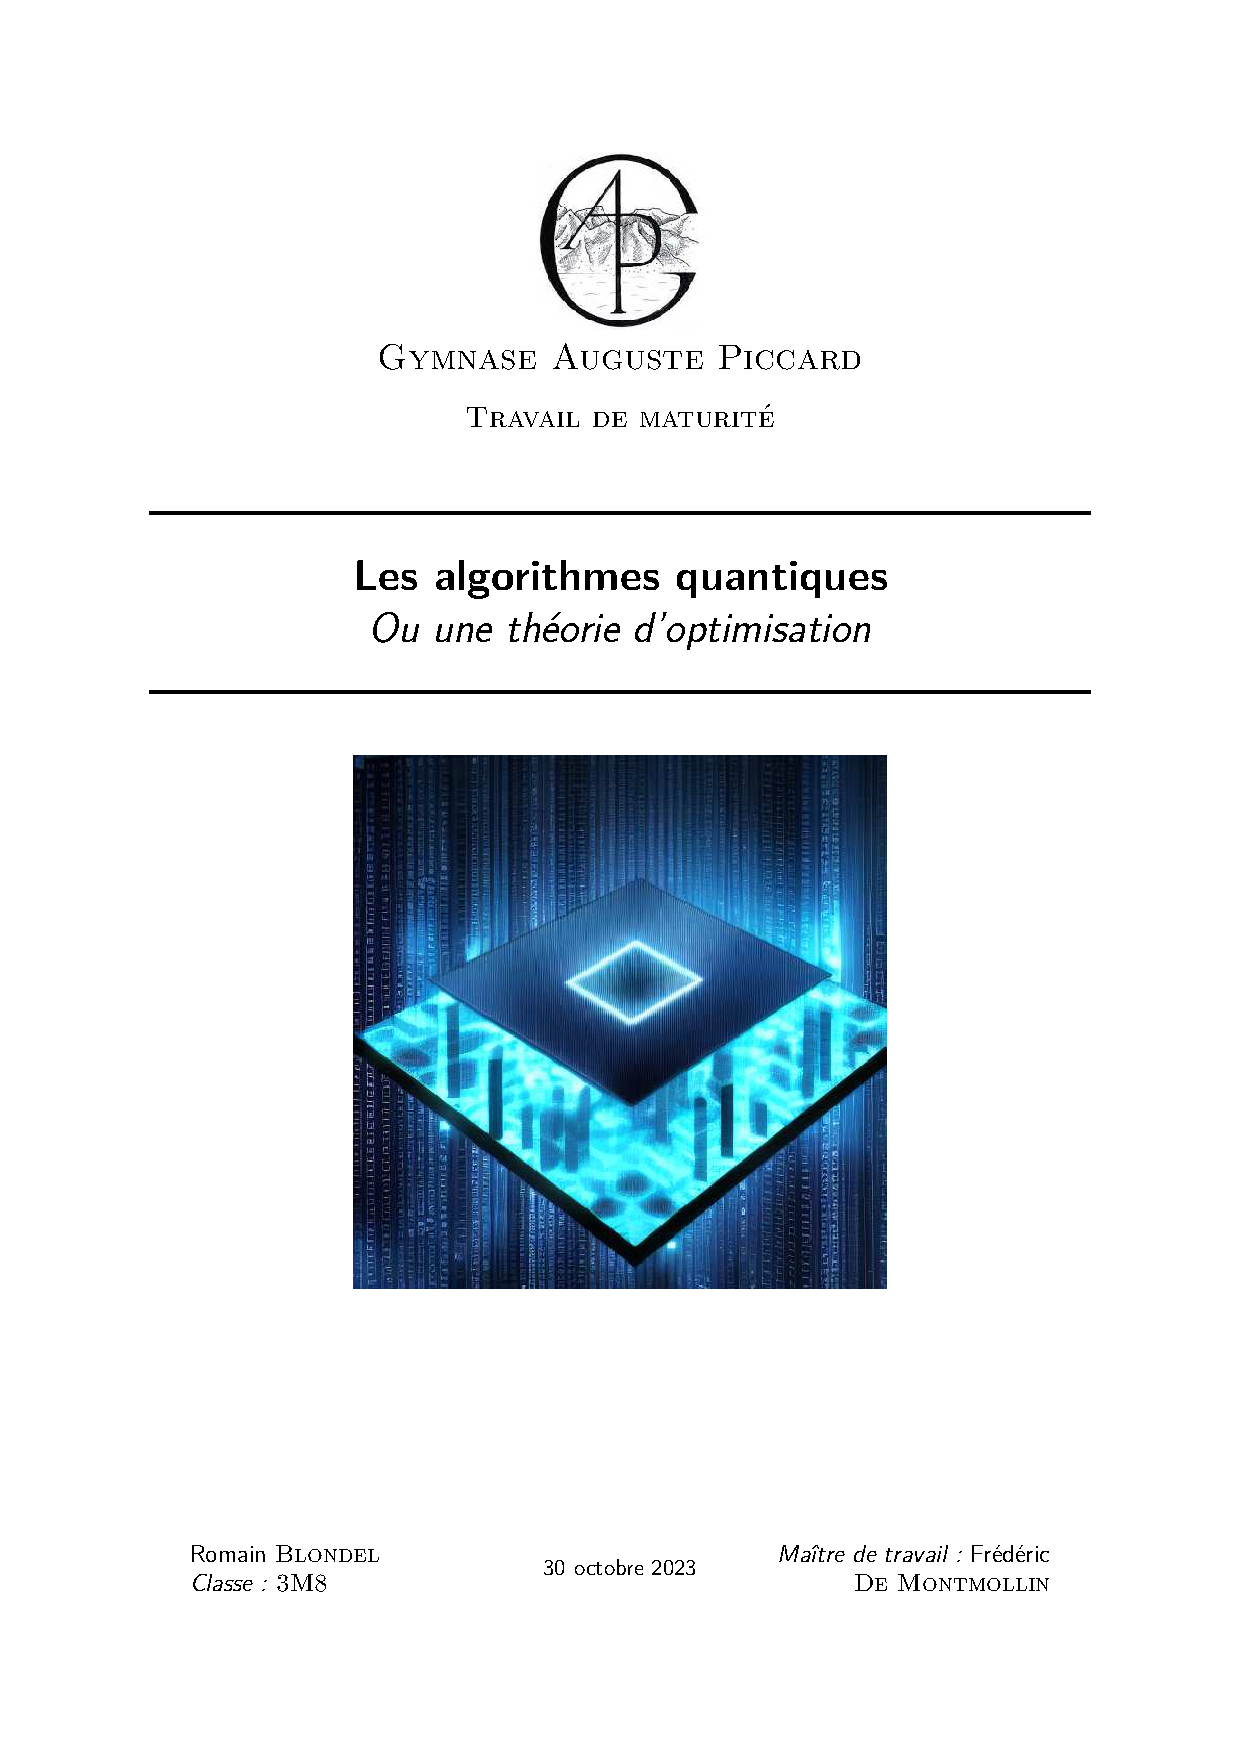
\includegraphics[height = 0.3\textwidth]{Blondel_romain_lesalgorithmesquantiques-ouunetheoriedoptimisation-1.pdf}	
%\end{figure}

%% else use the following coding to input the bibitems directly in the
%% TeX file.

%%\begin{thebibliography}{00}

%% \bibitem[Author(year)]{label}
%% For example:

%% \bibitem[Aladro et al.(2015)]{Aladro15} Aladro, R., Martín, S., Riquelme, D., et al. 2015, \aas, 579, A101


%%\end{thebibliography}

\end{document}

\endinput
%%
%% End of file `elsarticle-template-harv.tex'.
